\documentclass[11pt]{article}
\usepackage{amsmath,amssymb,amsthm}
\usepackage{tikz}
\usepackage{hyperref}
\usepackage[margin=1in]{geometry}

\newcommand{\N}{\mathbb{N}}
\newcommand{\Z}{\mathbb{Z}}
\newcommand{\Q}{\mathbb{Q}}
\newcommand{\La}{\Lambda}
\newcommand{\GK}{\operatorname{GK}}
\newcommand{\CPP}{\operatorname{CPP}}
\newcommand{\ALCD}{\operatorname{ALCD}}
\newcommand{\IP}{\operatorname{IP}}
\newcommand{\qpoch}[2]{(#1;#2)_\infty}
\newcommand{\qpochn}[3]{(#1;#2)_{#3}}
\newcommand{\qbin}[2]{\genfrac{[}{]}{0pt}{}{#1}{#2}}
\DeclareMathOperator{\tr}{tr}
\DeclareMathOperator{\wt}{wt}
\DeclareMathOperator{\sgn}{sgn}

\theoremstyle{plain}
\newtheorem{theorem}{Theorem}
\newtheorem{conjecture}[theorem]{Conjecture}
\newtheorem{proposition}[theorem]{Proposition}
\newtheorem{lemma}[theorem]{Lemma}
\newtheorem{corollary}[theorem]{Corollary}
\theoremstyle{definition}
\newtheorem{definition}[theorem]{Definition}
\newtheorem{example}[theorem]{Example}
\newtheorem{remark}[theorem]{Remark}

\title{$Q$-Non-Intersecting Lattice Paths}
\author{Robin Langer}
\date{\today}

\begin{document}
\maketitle

\begin{abstract}
We develop the $Q$-enriched lattice path model for cylindric
plane partitions.  In the standard model~\cite{langer-thesis},
CPPs biject with families of non-intersecting lattice paths
on the cylinder.  We define a \emph{$Q$-lattice path family}
as a pair $(S, \mathfrak{p})$, where $\mathfrak{p}$ is a
non-intersecting family and $S$ records crossing positions.
When $S = \emptyset$ the family is non-intersecting and
corresponds to a CPP; when $S \neq \emptyset$ the paths
cross and the family carries sign $(-1)^{|S|}$.
The positivity of $Q_{n,c}(q)$ becomes the statement that
all intersecting families can be cancelled by a
sign-reversing involution, leaving only non-intersecting
(CPP) contributions.
\end{abstract}

\tableofcontents


%% ============================================================
\section{The standard NILP model}
\label{sec:standard}
%% ============================================================

We recall the bijection between cylindric plane partitions and
non-intersecting lattice paths (NILPs) on the
cylinder~\cite{langer-thesis}.

\subsection{Paths on the cylinder}

A \emph{lattice path} on a cylinder of period~$T$ is a
sequence $p = (y_0, y_1, \ldots, y_T)$ of integers with
$y_{k+1} - y_k \in \{0, 1\}$ for each~$k$.  Each step is
either:
\begin{itemize}
  \item \textbf{Up}: $y_{k+1} = y_k + 1$ (encoded as $1$),
  \item \textbf{Flat}: $y_{k+1} = y_k$ (encoded as $0$).
\end{itemize}
The path is encoded by the binary string
$p = (p_0, \ldots, p_{T-1})$ and a starting height~$y_0$.


\subsection{Non-intersecting families}

\begin{definition}[NILP family]
\label{def:NILP}
A \emph{family of non-intersecting lattice paths} on the
cylinder of period~$T$ is a collection of paths
$p^1, p^2, \ldots, p^m$ satisfying:
\begin{enumerate}
  \item $y_k^{i+1} > y_k^i$ for all $k$ and $i$
    \textup{(non-intersecting)},
  \item $y_0^{i+1} - y_0^i = y_T^{i+1} - y_T^i$ for all~$i$
    \textup{(cylindric closure)}.
\end{enumerate}
\end{definition}


\subsection{The CPP--NILP bijection}

\begin{theorem}[{\cite{langer-thesis}, Theorem~4.2}]
\label{thm:NILP-bijection}
Let $\pi$ be a binary string of length~$T$.  There is a
bijection between cylindric plane partitions of profile~$\pi$
and minimal families of non-intersecting lattice paths on
the cylinder of period~$T$ with profile~$\pi$.

The bijection is given by the \emph{column-length encoding}:
the $i$-th path encodes the $i$-th column length across
successive partitions:
\begin{equation}\label{eq:column-path}
  \boxed{\;
  p_i(\mathfrak{c})_k
  = (\mu^{k+1})'_i - (\mu^k)'_i + \pi_k
  \;\in\; \{0, 1\},
  \;}
\end{equation}
where $\mathfrak{c} = (\mu^0, \mu^1, \ldots, \mu^T)$ is the
interlacing sequence and $(\mu^k)'_i$ is the length of the
$i$-th column of~$\mu^k$.
\end{theorem}


\subsection{Cubes}

\begin{definition}[Cube]
\label{def:cube}
A \emph{cube} in the NILP model is a pair of vertices
$v_1 = (x, y_1)$ and $v_2 = (x, y_2)$ at the same
$x$-coordinate with $y_1 < y_2$, where $v_1$ is
\emph{occupied} (lies on some path~$p^i$) and $v_2$ is
\emph{unoccupied} (lies between paths $p^j$ and $p^{j+1}$
for some~$j \geq i$).
\end{definition}

In the standard model, each cube carries weight~$1$, and the
total weight of a NILP family is the number of cubes.  This
equals the total weight $|\mathfrak{c}|$ of the corresponding
CPP\@.


\subsection{Three models}

We now have three equivalent models for the same objects:
\begin{center}
\begin{tabular}{l|l|l}
\textbf{Model} & \textbf{Object} & \textbf{Local structure}
  \\ \hline
Interlacing sequence &
  $(\mu^0, \mu^1, \ldots, \mu^T)$ &
  horizontal strips $\mu^k / \mu^{k-1}$ \\
Growth diagram &
  ALCD with face labels &
  local rule at each face \\
Lattice paths &
  non-intersecting paths &
  cubes (occupied--unoccupied pairs)
\end{tabular}
\end{center}

The growth diagram and lattice path models are
\emph{dual}: the growth diagram operates on
\emph{rows} of the partition (via Pieri operators $P_m$,
$T_n$), while the lattice paths track \emph{columns}.
The cube in the NILP model corresponds to the face label in
the growth diagram.


%% ============================================================
\section{$Q$-weighted lattice paths}
\label{sec:Q-paths}
%% ============================================================

We now enrich the NILP model with $Q$-weights.


\subsection{Strip sizes in the NILP picture}

At step~$k$ of the interlacing sequence
$\mathfrak{c} = (\mu^0, \mu^1, \ldots, \mu^T)$, the
horizontal strip $\mu^k / \mu^{k-1}$ (or
$\mu^{k-1} / \mu^k$, depending on $\pi_k$) has size
$a_k = ||\mu^k| - |\mu^{k-1}||$.

In the NILP picture, the strip size~$a_k$ equals the number of
paths that take an ``up'' step at position~$k$ minus the number
expected from the profile:
\begin{equation}\label{eq:strip-NILP}
  a_k = \#\{i : p_i(\mathfrak{c})_k = 1\} - \pi_k
    \cdot (\text{number of paths}).
\end{equation}
More precisely, $a_k$ is the number of \emph{free} up-steps
at position~$k$ (those not forced by the profile).


\subsection{$Q$-weight of a cube}

\begin{definition}[$Q$-cube weight]
\label{def:Q-cube}
Let $c = (v_1, v_2)$ be a cube at $x$-coordinate~$k$, with
$v_1$ on path~$p^i$ and $v_2$ between paths $p^j$ and
$p^{j+1}$.  The \emph{$Q$-weight} of~$c$ depends on the
strip sizes at position~$k$:
\begin{equation}\label{eq:Q-cube-weight}
  \wt_Q(c) = Q_{a_k(c)}(q),
\end{equation}
where $a_k(c)$ is the strip size at position~$k$ as seen from
the cube~$c$ (i.e., the local strip size involving the paths
between $p^i$ and $p^{j+1}$).
\end{definition}

In the standard model, $Q_n = 1$ for all~$n$ (i.e., $d = 1$),
so all cubes carry weight~$1$.  For $d \geq 2$, the $Q$-weight
depends on the geometric context of the cube within the path
family.


\subsection{$Q$-weighted NILP families}

\begin{definition}[$Q$-NILP]
\label{def:Q-NILP}
A \emph{$Q$-weighted non-intersecting lattice path family}
(or $Q$-NILP) is a standard NILP family where each cube~$c$
carries the $Q$-weight~\eqref{eq:Q-cube-weight}.  The total
$Q$-weight of the family is the product over all cubes:
\begin{equation}\label{eq:total-Q-weight}
  \wt_Q(\mathfrak{c})
  = \prod_{\text{cubes } c \text{ in } \mathfrak{c}}
    Q_{a(c)}(q).
\end{equation}
\end{definition}


%% ============================================================
\section{The $Q$-kernel as a two-path interaction}
\label{sec:two-path}
%% ============================================================

The lattice path picture gives a geometric interpretation of
the $Q$-kernel $\Phi_{a,b}(t)$.

\subsection{Two adjacent paths}

Consider two adjacent paths $p^i$ and $p^{i+1}$ in a NILP
family.  At each $x$-coordinate~$k$, each path takes an up or
flat step.  There are four possibilities:
\begin{center}
\begin{tabular}{c|c|l}
$p^i_k$ & $p^{i+1}_k$ & \textbf{Interaction} \\ \hline
$0$ (flat) & $0$ (flat) &
  paths maintain gap; no cube created \\
$1$ (up) & $1$ (up) &
  paths maintain gap; no cube created \\
$0$ (flat) & $1$ (up) &
  gap increases by $1$; no cube created \\
$1$ (up) & $0$ (flat) &
  gap decreases by $1$; \textbf{cube created}
\end{tabular}
\end{center}

A cube between $p^i$ and $p^{i+1}$ is created precisely when
$p^i$ goes up and $p^{i+1}$ stays flat.  In the growth diagram
language, this corresponds to a face with label $k \geq 1$:
the cascade parameter counts the number of ``crossings''
where the lower path rises into the territory of the upper
path.


\subsection{The cascade as gap reduction}

At cascade level~$k$, the two-path interaction has the lower
path taking $k$ more up-steps than the upper path over the
same interval.  Each such up-step creates a cube.  The
$Q$-weight of the $j$-th cube is $Q_{a+j}(q)$ (for the lower
path) times $Q_{b+j}(q)$ (for the upper path), where $a$ and
$b$ are the initial strip sizes.

The $Q$-kernel is the generating function for these
interactions:
\begin{equation}\label{eq:Phi-NILP}
  \boxed{\;
  \Phi_{a,b}(t)
  = \sum_{k \geq 0} Q_{a+k}\, Q_{b+k}\, t^k
  = \sum_{\substack{\text{two-path} \\
    \text{interactions}}}
    \wt_Q \cdot t^{\#\text{cubes}}.
  \;}
\end{equation}


\subsection{The shifted factorisation, geometrically}

The shifted factorisation
$\Phi_{a,b}(t) = Q_a\, Q_b + t\,\Phi_{a+1,b+1}(t)$
has a geometric meaning in the NILP picture:
\begin{itemize}
  \item $Q_a \cdot Q_b$: no cubes between the two paths
    ($k = 0$).  The paths maintain their gap throughout.
    The $Q$-weight is the product of the individual
    path weights.
  \item $t \cdot \Phi_{a+1,b+1}(t)$: at least one cube is
    created ($k \geq 1$).  The first cube has
    $Q$-weight $Q_{a+1} \cdot Q_{b+1}$, and the remaining
    cubes contribute $\Phi_{a+1,b+1}(t)$.  The factor
    $t$ records the first cube.
\end{itemize}
Peeling off one cube at a time is exactly the layer-by-layer
structure of the peel/glue involution
(\cite{LOCAL_RULE}, Section~7).


%% ============================================================
\section{$Q$-lattice path families}
\label{sec:Q-families}
%% ============================================================

We now define the central object: a $Q$-lattice path family.
This is a pair $(S, \mathfrak{p})$ --- not just a NILP
family~$\mathfrak{p}$ --- and the subset~$S$ records where
paths \emph{cross}.

\subsection{Pairs as path families with crossings}

\begin{definition}[$Q$-lattice path family]
\label{def:Q-lattice-path}
A \emph{$Q$-lattice path family} of level~$n$ and
profile~$c$ is a pair $(S, \mathfrak{p})$ where:
\begin{itemize}
  \item $\mathfrak{p}$ is a NILP family of $n - |S|$
    non-intersecting paths on the cylinder,
  \item $S \subseteq \{1, \ldots, n\}$ is the set of
    \emph{crossing positions},
  \item sign: $(-1)^{|S|}$,
  \item weight: $q^{\sigma(S) + |\mathfrak{p}|}$ where
    $\sigma(S) = \sum_{i \in S} i$.
\end{itemize}
\end{definition}

This is the lattice path incarnation of the ground-set
element $(S, \mathfrak{d}) \in \mathcal{G}_{n,c}$: the
ALCD~$\mathfrak{d}$ corresponds to the NILP
family~$\mathfrak{p}$, and the subset~$S$ records the
crossing positions.


\subsection{Non-intersecting vs.\ intersecting families}

The two cases carry fundamentally different combinatorial
meaning:

\begin{itemize}
  \item \textbf{$S = \emptyset$} (non-intersecting):
    The pair $(\emptyset, \mathfrak{p})$ is a genuine NILP
    family of~$n$ non-intersecting paths.  Under the
    CPP--NILP bijection (Theorem~\ref{thm:NILP-bijection}),
    this corresponds to a \emph{cylindric plane partition}.
    Sign:~$+1$.

  \item \textbf{$S \neq \emptyset$} (intersecting):
    The pair $(S, \mathfrak{p})$ represents a path
    configuration where $|S|$ crossings have occurred.
    The NILP family~$\mathfrak{p}$ has only $n - |S|$
    non-intersecting paths; the elements of~$S$ mark the
    levels at which paths have crossed.  This does
    \emph{not} correspond to a CPP\@.
    Sign:~$(-1)^{|S|}$.
\end{itemize}

Every CPP of level~$n$ gives a non-intersecting family
$(\emptyset, \mathfrak{p})$.  But a general $Q$-lattice
path family $(S, \mathfrak{p})$ with $S \neq \emptyset$
represents an \emph{intersecting} configuration --- and
these are precisely what the involution must cancel.


\subsection{What are intersecting paths?}
\label{sec:what-intersecting}

In the CPP world, every cylindric plane partition corresponds to a
non-intersecting lattice path configuration.  There are no
``intersecting CPPs.''  So where do the intersecting $Q$-lattice
path families live?

They live in a \emph{larger space} than the CPP space.
In the multipartition representation, a CPP with profile
$c = (c_0, c_1, c_2)$ and max entry~$n$ is a triple of partitions
$(\nu^1, \nu^2, \nu^3)$ satisfying the cyclic interlacing conditions
at every level $s = 1, \ldots, n$:
\begin{equation}\label{eq:interlacing}
  \nu^1_s \geq \nu^2_{s+c_1}, \qquad
  \nu^2_s \geq \nu^3_{s+c_2}, \qquad
  \nu^3_s \geq \nu^1_{s+c_0}.
\end{equation}
These conditions encode the non-intersecting property: at each
level~$s$, the three lattice paths maintain their relative order on
the cylinder.

A $Q$-lattice path family $(S, \mathfrak{p})$ with
$S \neq \emptyset$ corresponds to a path configuration where the
interlacing conditions~\eqref{eq:interlacing} are
\emph{relaxed} at the levels in~$S$:
\begin{itemize}
  \item At levels $s \notin S$: the interlacing holds
    (paths maintain order $\Rightarrow$ non-intersecting).
  \item At levels $s \in S$: the interlacing may fail
    (paths cross $\Rightarrow$ intersection at level~$s$).
\end{itemize}

\begin{remark}[The enlarged path space]
\label{rem:enlarged}
The ground set $\mathcal{G}_{n,c}$ is the enlarged path
space: the set of all path configurations on the cylinder---both
non-intersecting and intersecting---indexed by
$(S, \mathfrak{p})$.  For $S = \emptyset$, we recover the CPP
space.  For $S \neq \emptyset$, we get configurations outside
the CPP space: triples of partitions where the cylindric closure
condition fails at the levels in~$S$.

This parallels the classical LGV setup:
\begin{itemize}
  \item The LGV determinant sums over \emph{all} path families
    (all permutations $\sigma \in S_r$).
  \item The identity permutation gives non-intersecting paths.
  \item Other permutations give intersecting paths.
  \item The involution cancels intersecting paths, leaving
    only non-intersecting ones.
\end{itemize}
The $Q$-lattice path framework does the same, but the ``all path
families'' are indexed by subsets $S \subseteq \{1, \ldots, n\}$
(recording \emph{where} paths cross) rather than by permutations
$\sigma \in S_r$ (recording \emph{which} paths cross).
\end{remark}


\subsection{The $Q$-polynomial as a signed path count}

The $Q$-polynomial is the signed generating function over
all $Q$-lattice path families:
\begin{equation}\label{eq:Q-signed}
  \boxed{\;
  Q_n = \sum_{(S, \mathfrak{p}) \in \mathcal{G}_{n,c}}
    (-1)^{|S|}\, q^{\sigma(S) + |\mathfrak{p}|}.
  \;}
\end{equation}
The non-intersecting families ($S = \emptyset$) contribute
with sign~$+1$.  The intersecting families
($S \neq \emptyset$) contribute with alternating signs based
on the number of crossings.  Warnaar's conjecture states
that the positive contributions dominate.


%% ============================================================
\section{The Euler factor and crossings}
\label{sec:euler}
%% ============================================================

The crossings in a $Q$-lattice path family arise from the
Euler factor in the E--H factorisation.


\subsection{How crossings arise}

The $Q$-polynomial comes from:
\[
  Q_n = (q)_n \cdot [z^n]\, \bigl(\qpoch{zq}{q}\,
  \GK_c(z,q)\bigr).
\]
The factor $\GK_c(z,q)$ counts CPPs --- equivalently,
\emph{non-intersecting} NILP families.  The Euler factor
$\qpoch{zq}{q} = \prod_{i \geq 1}(1 - zq^i)$ relaxes
the non-intersecting condition by introducing crossings:
each factor $(1 - zq^i)$ either
\begin{itemize}
  \item leaves the family unchanged ($\times\, 1$), or
  \item introduces a \emph{crossing} at level~$i$
    ($\times\, (-zq^i)$).
\end{itemize}
Choosing $j$ crossing levels
$1 \leq \ell_1 < \cdots < \ell_j$ contributes
$(-z)^j q^{\ell_1 + \cdots + \ell_j}$.  Summing over all
choices:
\[
  \sum_{1 \leq \ell_1 < \cdots < \ell_j}
    q^{\ell_1 + \cdots + \ell_j}
  = \frac{q^{j(j+1)/2}}{(q)_j},
\]
recovering Euler's identity
$\qpoch{zq}{q} = \sum_{j \geq 0}
  \frac{(-1)^j z^j q^{j(j+1)/2}}{(q)_j}$.


\subsection{The $q$-binomial decomposition in path language}

Combining the Euler factor with $\GK_c$ and extracting
$[z^n]$:
\begin{equation}\label{eq:q-binom-decomp}
  Q_n = \sum_{j=0}^{n} (-1)^j\, q^{j(j+1)/2}\,
    \qbin{n}{j}\, h_{n-j},
\end{equation}
where $h_m = (q)_m \cdot [z^m]\,\GK_c(z,q) \in \N[q]$.

In path language, each term has a concrete meaning:
\begin{itemize}
  \item $n$ path levels, of which $j$ have crossings and
    $n - j$ are non-intersecting,
  \item $(-1)^j$: sign from $j$ crossings,
  \item $q^{j(j+1)/2}$: minimum crossing weight (crossings
    at the lowest possible levels $1, 2, \ldots, j$),
  \item $\qbin{n}{j}$: ways to arrange $j$ crossings among
    $n$ levels, with $q$-weight from their positions,
  \item $h_{n-j}$: $Q$-weighted count of the $n-j$
    non-intersecting paths.
\end{itemize}


%% ============================================================
\section{The crossing involution}
\label{sec:crossing-invol}
%% ============================================================

The sign-reversing involution $\iota$ on
$\mathcal{G}_{n,c}$~(\cite{LOCAL_RULE}) has a concrete
path interpretation: it \emph{introduces} or \emph{resolves}
crossings in a $Q$-lattice path family.


\subsection{Introducing and resolving crossings}

\begin{definition}[Crossing operations]
\label{def:crossing-ops}
Given a $Q$-lattice path family $(S, \mathfrak{p})$:
\begin{itemize}
  \item \textbf{Introduce a crossing} (peel): extract a
    path from~$\mathfrak{p}$ at level~$\ell$ using the
    inverse local rule.  The path collapses into a crossing
    at~$\ell$:
    \[
      (S, \mathfrak{p}) \;\xrightarrow{\;\text{peel}\;}
      (S \cup \{\ell\},\; \mathfrak{p}').
    \]
    One fewer non-intersecting path, one more crossing.
    Sign reverses.

  \item \textbf{Resolve a crossing} (glue): take a
    crossing at position $i \in S$ and re-insert a path
    at level~$i$ using the forward local rule:
    \[
      (S, \mathfrak{p}) \;\xrightarrow{\;\text{glue}\;}
      (S \setminus \{i\},\; \tilde{\mathfrak{p}}).
    \]
    One more non-intersecting path, one fewer crossing.
    Sign reverses.
\end{itemize}
\end{definition}


\subsection{Two directions for crossings}

The inverse local rule has two cascade directions:
\begin{itemize}
  \item \textbf{Burge} (cascade up): crosses the path
    from below,
  \item \textbf{RSK} (cascade down): crosses the path
    from above.
\end{itemize}
The paired involution compares the Burge crossing
candidate~$\ell_B$ with the RSK crossing candidate~$\ell_R$
and acts on whichever wins the Franklin-style
comparison~(\cite{LOCAL_RULE}, Section~13).


\subsection{Geometry: crossing and uncrossing}

\begin{center}
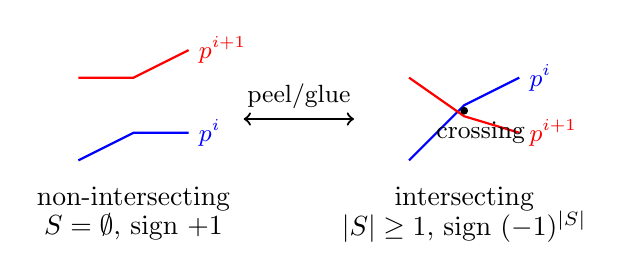
\begin{tikzpicture}[scale=0.7]
  %% Non-intersecting (left)
  \draw[thick,blue] (0,0) -- (1,0.5) -- (2,0.5)
    node[right]{\small $p^i$};
  \draw[thick,red] (0,1.5) -- (1,1.5) -- (2,2)
    node[right]{\small $p^{i+1}$};
  \node at (1,-0.7) {non-intersecting};
  \node at (1,-1.2) {$S = \emptyset$, sign $+1$};

  %% Arrow
  \draw[thick,<->] (3,0.75) -- (5,0.75)
    node[midway,above]{\small peel/glue};

  %% Intersecting (right)
  \draw[thick,blue] (6,0) -- (7,1) -- (8,1.5)
    node[right]{\small $p^i$};
  \draw[thick,red] (6,1.5) -- (7,0.8) -- (8,0.5)
    node[right]{\small $p^{i+1}$};
  \fill (7,0.9) circle (2pt);
  \node at (7.3,0.5) {\small crossing};
  \node at (7,-0.7) {intersecting};
  \node at (7,-1.2) {$|S| \geq 1$, sign $(-1)^{|S|}$};
\end{tikzpicture}
\end{center}

The peel operation converts a non-intersecting pair of
paths into an intersecting one (introducing a crossing);
the glue operation resolves a crossing back into a
non-intersecting configuration.  The involution~$\iota$
pairs these two types.


%% ============================================================
\section{Positivity as cancellation of crossings}
\label{sec:positivity}
%% ============================================================

Warnaar's Conjecture~2.7 states $Q_n \in \Z_{\geq 0}[q]$.
In the $Q$-lattice path framework, this is a statement
about the cancellation of intersecting families.

\begin{conjecture}[Path form]
\label{conj:path}
The signed sum~\eqref{eq:Q-signed} over $Q$-lattice path
families of level~$n$ has non-negative coefficients.
Equivalently: all intersecting families ($S \neq \emptyset$)
can be cancelled by the sign-reversing involution~$\iota$,
leaving only non-intersecting families ($S = \emptyset$).
\end{conjecture}

\begin{proposition}
\label{prop:non-intersecting-survive}
If every intersecting $Q$-lattice path family
($|S| \geq 1$) is paired by~$\iota$ with a family of
opposite sign, then:
\[
  Q_n = \sum_{\substack{(\emptyset, \mathfrak{p}) \\
    \text{fixed by } \iota}}
    q^{|\mathfrak{p}|}
  \;\in\; \Z_{\geq 0}[q].
\]
That is: $Q_n$ counts exactly the non-intersecting
$Q$-weighted NILP families that survive the cancellation
of all intersecting families.
\end{proposition}

\begin{remark}[Why positivity is natural]
\label{rem:why-positive}
The path picture makes positivity intuitively plausible.
An intersecting family has paths that cross, and a crossing
can typically be resolved by ``uncrossing'' the offending
pair.  The non-intersecting condition constrains which
crossings can occur, and for most configurations, a
sign-reversing partner exists.  The rare configurations
that survive --- the genuine non-intersecting families ---
contribute positively.
\end{remark}

\begin{remark}[Rank~$3$ constraint]
\label{rem:rank3}
For rank~$3$, the cylinder has circumference~$T = d$ and
the NILP families have at most~$3$ paths.  The crossing
structure is therefore very constrained: at most two
adjacent pairs of paths can cross.  This small size is
what makes the conjecture tractable.
\end{remark}


%% ============================================================
\section{The $Q$-kernel and paired crossings}
\label{sec:paired-crossings}
%% ============================================================

For the pair set $\mathcal{P}_{a,b,k}
= \mathcal{G}_{a+k} \times \mathcal{G}_{b+k}$, the NILP
interpretation involves \emph{two} $Q$-lattice path
families coupled at cascade level~$k$.

\begin{definition}[$Q$-NILP pair]
\label{def:Q-NILP-pair}
A \emph{$Q$-NILP pair} at cascade level~$k$ with strip
sizes $(a,b)$ is a pair of $Q$-lattice path families:
\[
  \bigl((S, \mathfrak{p}),\; (S', \mathfrak{p}')\bigr)
  \;\in\;
  \mathcal{G}_{a+k,c} \times \mathcal{G}_{b+k,c}.
\]
The first family has level $a + k$; the second has level
$b + k$.  The cascade parameter~$k$ couples them.
\end{definition}

The $Q$-kernel $\Phi_{a,b}(t)$ is the signed generating
function of $Q$-NILP pairs:
\begin{equation}\label{eq:Phi-NILP-pairs}
  \Phi_{a,b}(t) = \sum_{k \geq 0} t^k
    \sum_{\substack{(S, \mathfrak{p}) \in
      \mathcal{G}_{a+k} \\
      (S', \mathfrak{p}') \in \mathcal{G}_{b+k}}}
    (-1)^{|S|+|S'|}\,
    q^{\sigma(S)+|\mathfrak{p}|+\sigma(S')+|\mathfrak{p}'|}.
\end{equation}

The paired involution $\iota$~(\cite{LOCAL_RULE},
Section~13) becomes a \emph{coupled crossing operation}:
introduce a crossing in one family (Burge direction) or
the other (RSK direction), comparing the two crossing
candidates to decide which family to act on.


%% ============================================================
\section{The LGV perspective}
\label{sec:LGV}
%% ============================================================

The Lindstr\"om--Gessel--Viennot lemma gives a
determinantal expression for the generating function
of NILP families.

\subsection{Standard LGV}

For sources $A = (a_1, \ldots, a_r)$ and sinks
$B = (b_1, \ldots, b_r)$ on a directed acyclic graph, the
LGV lemma states:
\begin{equation}\label{eq:LGV}
  \sum_{\text{NILPs } A \to B}
    \prod_i \wt(p^i)
  = \det\bigl(h(a_i, b_j)\bigr)_{1 \leq i,j \leq r},
\end{equation}
where $h(a, b)$ is the (weighted) generating function for
all paths from~$a$ to~$b$.

For the cylinder, the LGV lemma gives:
\begin{equation}\label{eq:LGV-cylinder}
  \GK_c(z,q) = \det\bigl(h_c(a_i, b_j; z, q)\bigr),
\end{equation}
where $h_c$ is the cylindric path generating function.


\subsection{$Q$-LGV}

In the $Q$-enriched setting, each path step carries a
$Q$-weight.  The $Q$-enriched path generating function is:
\begin{equation}\label{eq:Q-path-gf}
  h_c^Q(a, b; z, q)
  = \sum_{\text{paths } a \to b}
    \prod_{\text{steps}} Q_{a_k}(q) \cdot
    z^{\#\text{up-steps}} \cdot q^{\text{weight}}.
\end{equation}

\begin{proposition}[$Q$-LGV]
\label{prop:Q-LGV}
The $Q$-weighted NILP generating function is:
\begin{equation}\label{eq:Q-LGV}
  \sum_{\text{$Q$-NILPs}}
    \wt_Q \cdot z^{|\mathfrak{c}|}
  = \det\bigl(h_c^Q(a_i, b_j; z, q)\bigr).
\end{equation}
The $Q$-enrichment replaces the scalar entries of the LGV
matrix with $Q$-weighted path counts.
\end{proposition}

\begin{remark}[LGV and crossings]
\label{rem:LGV-crossings}
The LGV determinant naturally includes all path
families --- both non-intersecting and intersecting ---
with sign from the permutation.  Off-diagonal permutations
force paths to cross.  The $Q$-lattice path family
$(S, \mathfrak{p})$ refines this: $S$ tracks the
crossings explicitly, and the involution operates on
individual crossings rather than on permutations.
\end{remark}


\subsection{LGV crossings vs.\ $Q$-NILP crossings}
\label{sec:LGV-vs-QNILP}

The crossing structure in the $Q$-NILP framework differs
fundamentally from that in the classical LGV lemma:

\begin{center}
\begin{tabular}{l|l|l}
  & \textbf{Classical LGV} & \textbf{$Q$-NILP} \\ \hline
Crossing indexed by &
  $\sigma \in S_r$ &
  $S \subseteq \{1, \ldots, n\}$ \\
Meaning &
  which paths swap destinations &
  at which levels paths cross \\
Number of types &
  $r!$ (topological) &
  $2^n$ (geometric) \\
Sign &
  $\sgn(\sigma)$ &
  $(-1)^{|S|}$ \\
Involution &
  swap tails at first intersection &
  peel/glue at first crossing level \\
Fixed points &
  NILP (identity permutation) &
  non-intersecting $Q$-families \\
\end{tabular}
\end{center}

In the LGV framework, the permutation~$\sigma$ determines the
\emph{topology} of the crossing: which source connects to which
sink.  For rank~$3$, there are $3! = 6$ topological types.

In the $Q$-NILP framework, the subset~$S$ determines the
\emph{geometry} of the crossing: at which levels along the cylinder
the paths intersect.  For a family of level~$n$, there are $2^n$
geometric patterns.

Both decompositions express the same signed generating function.
However, the $Q$-NILP decomposition is \emph{finer}: it tracks
individual crossing events at each level rather than the global
crossing topology.  This finer granularity is what makes a
Franklin-style level-by-level involution possible.

\begin{remark}[Why subsets, not permutations?]
\label{rem:why-subsets}
In the classical LGV lemma on a directed acyclic graph (DAG), paths
are uniquely determined by their endpoints, so the crossing structure
is encoded by the endpoint permutation $\sigma \in S_r$.

On the \emph{cylinder}, paths can wind around, and the same pair
of endpoints can give rise to many different path families.  The
level-by-level structure of the growth diagram resolves this
multiplicity: each level is a separate commutation step, and the
subset $S$ records which steps involve crossings.  This is why the
$Q$-crossing data is a subset of $\{1, \ldots, n\}$
rather than a permutation.
\end{remark}


%% ============================================================
\section{Specialisations}
\label{sec:special}
%% ============================================================


\subsection{$d = 1$: standard NILPs}

When $d = 1$, $Q_n = 1$ for all~$n$.  Every cube carries
weight~$1$, and the $Q$-NILP model reduces to the standard
NILP model.  The LGV determinant gives the Borodin product
formula, and all intersecting families cancel perfectly.


\subsection{$d = 2$ (Rogers--Ramanujan): quadratic paths}

For $d = 2$ with $c = (2,0,0)$: $Q_n = q^{n^2}$.  Each
cube at strip size~$n$ carries weight $q^{n^2}$ --- a
quadratic function of the path position.  The NILP family
resembles paths in a quadratic potential.

The signed path count becomes:
\[
  Q_n = q^{n^2} = \sum_{(S, \mathfrak{p})}
    (-1)^{|S|}\, q^{\sigma(S) + |\mathfrak{p}|},
\]
which states that the intersecting families cancel so
completely that only a single monomial survives.  This
extreme cancellation reflects the Rogers--Ramanujan
structure.


\subsection{$d = 4$, $c = (2,2,0)$}

Here $Q_1 = q^2 + q^3 + q^4 + q^5$: a single cube can
carry four different weights.  The NILP picture shows
paths in a ``multi-well potential'' where each cube
position contributes a polynomial weight.  The
non-negativity of~$Q_n$ for all~$n$ means that all
intersecting families can be cancelled, despite the
complex weight structure.


%% ============================================================
\section{Connection to the pair framework}
\label{sec:connection}
%% ============================================================

The lattice path picture gives a geometric underpinning to
the pair-based involution programme of~\cite{LOCAL_RULE}:

\begin{center}
\begin{tabular}{l|l}
\textbf{Pair framework} &
  \textbf{NILP picture} \\ \hline
Ground-set element $(S, \mathfrak{d})$ &
  $Q$-lattice path family $(S, \mathfrak{p})$ \\
ALCD $\mathfrak{d}$ &
  Non-intersecting path family $\mathfrak{p}$ \\
Subset $S$ &
  Crossing positions \\
$S = \emptyset$ &
  Non-intersecting family (= CPP) \\
$S \neq \emptyset$ &
  Intersecting family (to be cancelled) \\
Peel (inverse rule) &
  Introduce a crossing \\
Glue (forward rule) &
  Resolve a crossing \\
Q-Burge (cascade up) &
  Cross from below \\
Q-RSK (cascade down) &
  Cross from above \\
Cascade parameter $k$ &
  Number of cubes between two paths \\
$Q$-kernel $\Phi_{a,b}(t)$ &
  Two-path interaction GF \\
Fixed points of $\iota$ &
  Non-intersecting families that survive
\end{tabular}
\end{center}


%% ============================================================
\section{Open questions}
\label{sec:open}
%% ============================================================

\begin{enumerate}
  \item \textbf{Explicit $Q$-LGV matrix.}\;
    Compute the $Q$-enriched LGV matrix for rank~$3$
    profiles.  The matrix entries $h_c^Q(a_i, b_j)$
    should be expressible in terms of the $Q_n$ and
    $q$-binomial coefficients.

  \item \textbf{Crossing involution.}\;
    Make the crossing involution explicit: given an
    intersecting $Q$-lattice path family
    $(S, \mathfrak{p})$ with $S \neq \emptyset$, specify
    which crossing to resolve (or which new crossing to
    introduce), using the non-intersecting condition as a
    guide.  The Burge direction (cross from below) and
    RSK direction (cross from above) give two options.

  \item \textbf{Fixed-point characterisation.}\;
    Characterise the fixed points of the crossing
    involution.  Are they always non-intersecting
    ($S = \emptyset$)?  If so, $Q_n$ counts genuine NILP
    families with $Q$-weighted cubes.

  \item \textbf{Rhombus tilings.}\;
    The NILP model is dual to rhombus tilings on the
    cylinder.  What does the $Q$-enrichment mean for
    tilings?  Each rhombus type would carry a $Q$-weight,
    and the tiling count becomes a $Q$-polynomial.

  \item \textbf{Cylinder circumference~$3$.}\;
    For rank~$3$, the cylinder has circumference~$T = d$
    and the NILP families have at most~$3$ paths with
    the LGV matrix being $3 \times 3$.  Work out the
    crossing structure explicitly for small~$n$ to see
    the cancellation in action.
\end{enumerate}


\begin{thebibliography}{99}
\bibitem{ADJOINT}
  R.~Langer,
  \emph{The $Q$-Operator and its Adjoint: From Level~3
  Operator Traces to Cascade Commutators},
  companion note, 2026.

\bibitem{Borodin}
  A.~Borodin,
  \emph{Periodic Schur process and cylindric partitions},
  Duke Math.~J.\ \textbf{140} (2007), 391--468.

\bibitem{LOCAL_RULE}
  R.~Langer,
  \emph{The Generalized Local Rule and the Burge--RSK
  Involution},
  companion note, 2026.

\bibitem{Q_SCHUTZ}
  R.~Langer,
  \emph{The $Q$-Sch\"utzenberger Identity},
  companion note, 2026.

\bibitem{langer-thesis}
  R.~Langer,
  \emph{Cylindric Partitions and Bijective Proofs},
  PhD thesis, University of Melbourne.

\bibitem{vanLeeuwen}
  M.~A.~A.~van~Leeuwen,
  \emph{The Robinson--Schensted and Sch\"utzenberger
  algorithms, an elementary approach},
  Electron.~J.~Combin.\ \textbf{3} (1996), R15.
\end{thebibliography}

\end{document}
